\documentclass{handout}

% \SetInstructor{Lt Col James Phillips}
\SetCourseTitle{ECE231: Electrical Circuits and Systems I}
\SetSemester{Block III}
\SetHandoutTitle{Lecture 28: Phasors and Impedance}

%\SetDueDate{1 Jan 2016}
%\ShowAllBlanks

\showsoln \setsolncolor{red}

\begin{document}
\maketitle

\textbf{OBJECTIVES:}
\begin{enumerate}
\item Understand what a Phasor is and how to do phasor math
\item Understand how to apply connection and device constraints with phasors
\item Understand the concept of impedance
\end{enumerate}

\textbf{READING}
\begin{description}
\item [Required]:
Textbook, section 8.1--8.2, pages 379--391
\item [Optional]:
\end{description}

\section{Introduction}
Over the next several lessons, we will start looking at {\em Steady-state Sinusoidal responses} of circuits.  Previously we have been looking at transient responses, so we are shifting gears a little bit.  In order to make our analysis easier, we will employee the technique of a phasor analysis.  What we will learn today is that a Phasor is just a way of representing a complex number and that they can make some of our math much easier.

\section{Phasor Basics}
To begin our look at phasors, we start with Euler's identity:
\[
e^{j\theta} = \cos \theta +j \sin \theta
\]
This is just a complex number of the form $a+jb$ but with a magnitude of 1.  We can mulitply  Euler's equation by a constant to represent any complex number:
\[
Ae^{j\theta} =A \cos \theta +j A\sin \theta
\]
From here we can recognize:
\soln{1.5in}{
\[
A\cos\theta = \mathbf{Re} [Ae^{j\theta}]
\]
\[
A\sin\theta = \mathbf{Im} [Ae^{j\theta}]
\]

}

This relationship is shown graphically in Figure \ref{fig: PhasorDiagram}

\begin{figure} [h!]
\centering
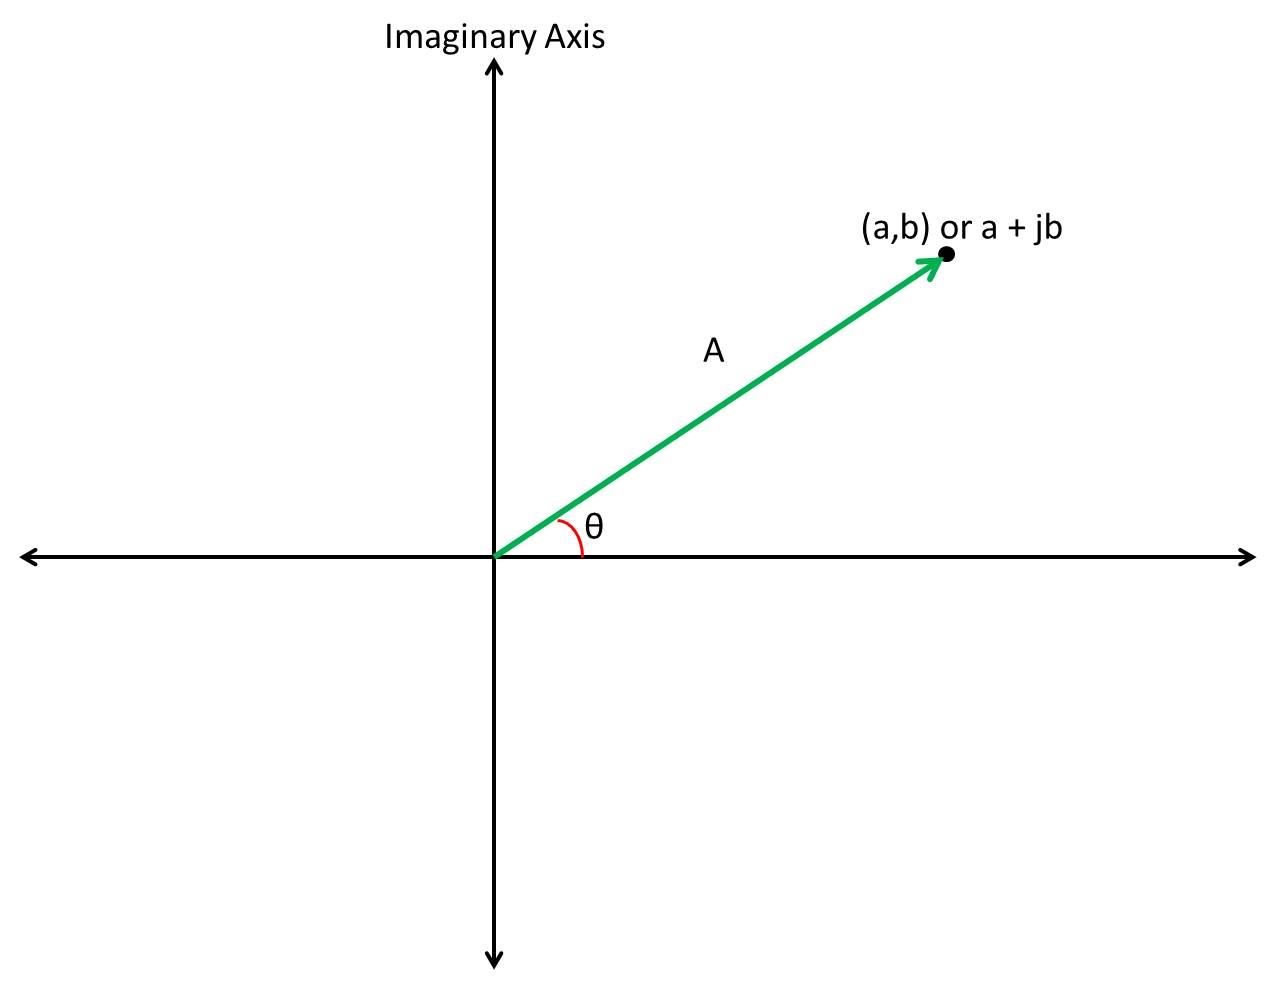
\includegraphics[width=0.75\textwidth]{PhasorDiagram.jpg}
\caption{Phasor Diagram}
\label{fig: PhasorDiagram}
\end{figure}

We can take advantage of this relationship to simplify some of our calculations.

What happens if we apply the equations above to a more general sinusoid like $A\cos(\omega t + \phi)$?

\soln{2in}{
\[
A\cos(\omega t + \phi) = A\mathbf{Re}\left[e^{j(\omega t +\phi)}\right]
\]
\[
A\mathbf{Re}\left[e^{j(\omega t +\phi)}\right]=A\mathbf{Re}\left[e^{j\omega t}e^{j\phi}\right]
\]
If we supress the $\mathbf{Re}$ and let $\mathbf{A} = Ae^{j\phi}$ we can rewrite this as
\[
A\mathbf{Re}\left[e^{j\omega t}e^{j\phi}\right] = \mathbf{A} e^{j\omega t}
\]

}

We call $\mathbf{A}$ the phasor representation of a  sinusoid.  Notice that the phasor carries information about the magnitude and phase of the sinusoid, but the frequency information is entirely supressed.  Also note that we could write $\mathbf{A}$ as
\[
\mathbf{A} = A\cos\phi+jA\sin\phi
\]
We can also use the following notation for $\mathbf{A}$
\[
\mathbf{A} = A\angle\phi
\]

\newpage
\clearpage
\pagebreak

\textbf{Example 1}--- Write the phasor representation of the following sinusoids (write in both polar and rectangular form):
\begin{itemize}
\item $20\cos(150t-60^\circ)$
\item $10\cos(1000t+180^\circ)$
\item $-4\cos 3t + 3\cos(3t-90^\circ)$
\end{itemize}

\soln{4in}{
\begin{figure} [h!]
\centering
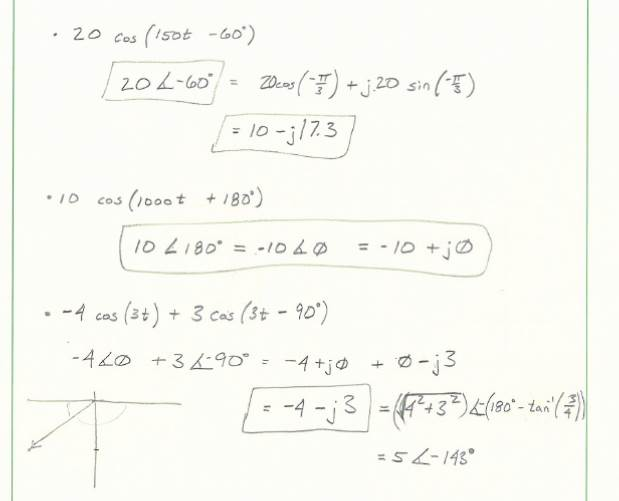
\includegraphics[width=0.6\textwidth]{Example1soln.jpg}
\end{figure}

}


\textbf{Example 2}---Convert the following phasors to sinusoids (assume $frequency = \omega$):
\begin{itemize}
\item $\mathbf{V} = 169 \angle -45^\circ$
\item $\mathbf{V} = 10 \angle 90^\circ + 66 -j10$
\item $\mathbf{I} = 15+j5+10\angle180^\circ$
\end{itemize}

\soln{4in}{
\begin{figure} [h!]
\centering
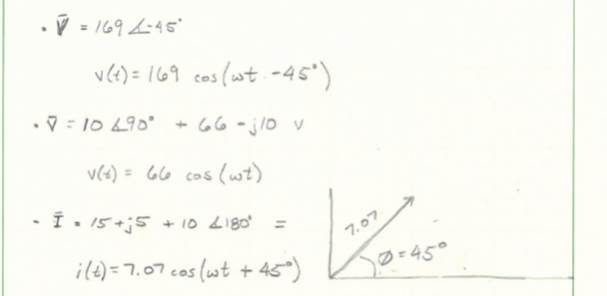
\includegraphics[width=0.75\textwidth]{Example2soln.jpg}
\end{figure}

}


\newpage
\clearpage
\pagebreak

\section{Important Properties of Phasors}
When using the following properties to analyze circuits it is important to always remember all our sinusoids (phasors) have to be the same frequency!  We are also only looking at steady state sinusoids!

\subsection{Additive Property}
If we have to phasors $\mathbf{A} = A\angle\phi_A$ and $\mathbf{B} = b\angle\phi_B$ and we want to add them, we must first convert to rectangular form:
\soln{2in}{
\[
A\angle\phi_A = A\cos\phi_A + jA\sin\phi_A
\]
\[
B\angle\phi_B = B\cos\phi_B + jB\sin\phi_B
\]
}

We can now use rules of complex addition to add these complex numbers
\soln{1in}{
\[
\mathbf{A} +\mathbf{B} = \left[A\cos\phi_A +B\cos\phi_B \right] +j\left[A\sin\phi_A+ B\sin\phi_B \right]
\]
}
Finally, we can convert back to polar form,

\textbf{Example 3} --Textbook Exercise 8-3.  Write the two signals below in phasor form, then add them.
\[i_1(t) = 100\cos\left(2000t\right)mA\]
\[i_2(t) = 50\cos\left(2000t-60^o\right)mA\]

\soln{4in}{
\[
\mathbf{I_1}=100\angle 0^o\ mA = 100 +j0\ mA
\]
\[
\mathbf{I_2}=50\angle -60^o\ mA = 25 -j43.3\ mA
\]
\[
\mathbf{I_1 +I_2} = \left[100 +25 \right] +j\left[0 -43.3 \right] = 125-j43.3\ mA
\]

To convert back to polar form
\[
|\mathbf{I_1 +I_2}|=\sqrt{125^2+(-43.3)^2}=132.3\ mA
\]
\[
\angle\mathbf{I_1 +I_2} = \tan^{-1}\left( \frac{-43.3}{125}\right) = -19.1^o
\]
Note: Be careful with the angle calculation... Depending on which quadrant you are in you the calculation can change... In quadrant 1 or 4, you can just take $\tan^{-1}$... In quadrant 2, you have to take $180^-\tan^{-1}$.... In quardrant 3, you will take $-(180^o-tan^{-1})$.  \textbf{Show some examples}
\[
\mathbf{I_1 +I_2} = 132.3\angle -19.1^o
\]

}
\newpage
\clearpage
\pagebreak
\subsection{Multiplication and Division}
Good News!  Multiplication and Division are a piece of cake with Phasors....

Recall that phasors are just complex exponentials and to multiply exponentials we follow the simple rule shown below:
\soln{1in}{
\[
Ae^{j\phi_A} \times Be^{j\phi_B} = ABe^{j(\phi_A+\phi_B)}
\]
}

So for phasors we can write:
\soln{1in}{
\[
A\angle\phi_A \times B\angle \phi_B = AB \angle \left( \phi_A +\phi_B \right)
\]
}

\textbf{Example 4}-- Multiply the following two phasors:
\[
\mathbf{A} = 10\angle 25^o
\]
\[
\mathbf{B} = 7\angle 15^o
\]
\soln{3in}{
\[
\mathbf{AB} = 7 \times 10 \angle \left( 25^o + 15^o\right) = 70\angle 40^o
\]
}

Division is very similar to mulitplication:
\soln{1in}{
\[
\frac{A\angle\phi_A}{B\angle\phi_B} = \frac{A}{B}\angle(\phi_A-\phi_B)
\]
}


\subsection{Derivative Property}
We have already seen that the derivative of a sinusoid is another sinusoid of the same frequency; this allows us to use phasors to describe their realationship.  Lets start by recalling that a sinusoid $v(t)$ is related to its phasor $\mathbf{V} = V\angle \phi_V$ by
\[
v(t) = \mathbf{Re}\left\{ \mathbf{V}e^{j\omega t} \right\}
\]

What happens when we take the time derivative of this expression?
\soln{2in}{
\[
\frac{\partial v(t)}{\partial t} = \frac{\partial}{\partial t} \mathbf{Re}\left\{ \mathbf{V}e^{j\omega t} \right\}
\]
The differntial on the right wide of the equation can be moved inside the $\mathbf{Re}$ and the derivative taken:
\[
\frac{\partial v(t)}{\partial t} = \mathbf{Re}\left\{\frac{\partial \mathbf{V}e^{j\omega t}}{\partial t}  \right\}
\]
This gives us
\[
\frac{\partial v(t)}{\partial t} =\mathbf{Re}\left\{j\omega \mathbf{V}e^{j\omega t}  \right\}
\]
Since for phasors we suppress the $\mathbf{Re}$ and the frequency dependence ($e^{j\omega t}$), we can take a derivatives in the phasor domain by just mulitplying by $j\omega$.

}

Given that we can take a derivative in the phasor domain by mulitplying by $j\omega$, we also know that:
\[
j\omega\mathbf{V} = \left(\omega e^{j90^o}\right)\left( V e^{j \phi} \right) = \omega  V e^{j (\phi + 90^o) }
\]

So the derivative scales the amplitude by $\omega$ and shifts the phase by $90^o$.


\newpage
\clearpage
\pagebreak

\section{Introduction to Circuit Analysis with Phasors}
In this section we will introduce how we can make circuit analysis easier by using phasors.  You have to remember that this analysis only applies to circuits that are excited by single frequency sinusoids and are in steady state.  This does not replace the transient analysis we have already learned.

\subsection{Connection Contraints}
As a reminder when we talk about connection constraints we are talking about \textbf{KVL} and \textbf{KCL}.  When we looked at circuits with sinusoidal forcing functions after they had reached steady state (natural response had decayed to zero), we observed that the forced response was also a sinusoid with the same frequency as the forcing function.  This means we could write a KVL equation around a loop that might look like:
\[
V_1\cos(\omega t +\phi_1) +V_2\cos(\omega t +\phi_2) + V_3\cos(\omega t +\phi_3) +..... = 0
\]

Where each voltage can have different amplitudes and phases, but they must have the same frequency, $\omega$.  If we were to write the equation above in phasor form we would get:

\soln{1in}{
\[
V_1\angle \phi_1+V_2\angle \phi_2+V_3\angle \phi_3+..... = 0
\]
}
This tells us that phasor voltages around a loop sum to zero; this is a phasor form of KVL.  You can also apply this to KCL; phasor current at a node must sum to zero.

\subsection{Device Constraints}
By device constraints we are referring to the $i$--$v$ characteristics of devices (resistors, capacitors and inductors).  Lets look at how phasor analysis might help us here. In the analysis below all currents and voltages are sinusoids with the following forms
\[
v(t) = \cos(\omega t +\phi)
\]
\[
i(t) = \cos (\omega t +\phi)
\]


\textbf{Resistors:}  The device contraint for resistors is just Ohm's law
\[
v_R(t) = i_R(t)R
\]
If we write this in Phasor form we get
\soln{1in}{
\[
V_R\angle \phi_V = I_R\angle \phi_I \times R
\]
}

It should be obvious that $\phi_V = \phi_I$, which means the voltage across a resistor and the current though the same resistor have the same phase angle (or are {\em in phase}).

\textbf{Capacitors} -- The device constraint for a capacitor is:
\[
i_c(t) = C\frac{\partial v_c(t)}{\partial t}
\]

If we use the derivative property to write this in phasor form we get:
\soln{2in}{
\[
I_c\angle \phi_I =  j\omega C V_c \angle \phi_V
\]
}
To make this look more like Ohm's law, lets solve for V:
\soln{2in}{
\[
V_c \angle \phi_V = \frac{1}{j\omega C}I_c\angle \phi_I
\]

Now for some mathemagic.... We know we can mulitply anything by 1 without changing the value.  We should also recognize that $-j^2 = 1$... If we mulitply $\frac{1}{j\omega C}$ by $-j^2$ we get:
\[
-j^2\times \frac{1}{j\omega C} = \frac{-j}{\omega C}=\frac{1}{\omega C}\angle -90^o
\]
plugging this back into our equation for $\mathbf{V_c}$ gives us
\[
V_c \angle \phi_V = \frac{I_c}{\omega C}\angle (\phi_I - 90^o)
\]
so
\[
\angle \phi_V = \angle (\phi_I - 90^o)
\]
}
This tells us that the phase of the voltage across a capacitor lags the current through that capacitor by $90^o$!

We can simplify the equation above by letting $\mathbf{V_c} = V_c\angle \phi_V$ and $\mathbf{I_c} = I_c\angle \phi_I$.  This allows us to write the equation more simply as:
\[
\mathbf{V_c}  = -\frac{j}{\omega C}\mathbf{I_c}
\]

\textbf{Inductors}-- The device constraint for an Inductor is:
\[
v_L(t) = L\frac{\partial i_L(t)}{\partial t}
\]
Like for our capacitor derivation we can use the derivative property to write this in phasor form we get:
\soln{2in}{
\[
V_L\angle \phi_V =j\omega L  I_L \angle \phi_I
\]
}

Similar to our capacitor development we should know that
\soln{1in}{
\[
j\omega L = \omega L \angle 90^o
\]
}

Plugging this into the equation above gives:
\soln{1in}{
\[
V_L\angle \phi_V =\omega L \angle 90^o  I_L \angle \phi_I=\omega L I_L \angle \left(\phi_I+90^o \right)
\]
}

This tells us that the phase of the voltage across a inductor leads the current through that inductor by $90^o$!

We can simplify the equation above by letting $\mathbf{V_L} = V_L\angle \phi_V$ and $\mathbf{I_L} = I_L\angle \phi_I$.  This allows us to write the equation more simply as:
\[
\mathbf{V_L}  = j\omega L\mathbf{I_L}
\]



A handy way to remember the current and voltage relationships in inductors and capacitors is to use the acronym {\em ELI the ICE man}.... $E$ leads $I$ in an inductor... $I$ leads $E$ in a capacitor.... In older texts books $E$ is used for voltage.
\newpage
\clearpage
\pagebreak
\section{Impedance}
We spent the last section deriving $i$--$v$ relationships in the phasor domain, but what has that really done for us?  If we look closely we will notice all the $i$--$v$ relationships in the above sections we will notice they all have the form:
\[
\mathbf{V} = \mathbf{I}Z
\]
where $\mathbf{V}$ and $\mathbf{I}$ are phasor voltage and current.

So for steady state sinusoidal circuits we can use a modified version of Ohm's law to analyze circuits with resistors, capacitors and inductors... No differential equations to be dealt with....

What is $Z$?  $Z$ is device impedence and is shown below for each circuit device:
\soln{2in}{
\[
Z_R = R
\]
\[
Z_C = -\frac{j}{\omega C} = \frac{1}{j\omega C}
\]
\[
Z_L = j\omega L
\]
}

Note: Impedances add just like resistances!

\subsection{Frequency  and Impedance}
From the equations above, it should be obvious that the impedance of a resistor is not affected by the fequency of the driving signal, however, the impedance of capacitors or inductors is affected.  To understand this effect, lets plot the impedance of a $1\ \mu F$ capacitor and a $500\ mH$ inductor:
\soln{4in}{
\begin{figure} [h!]
\centering
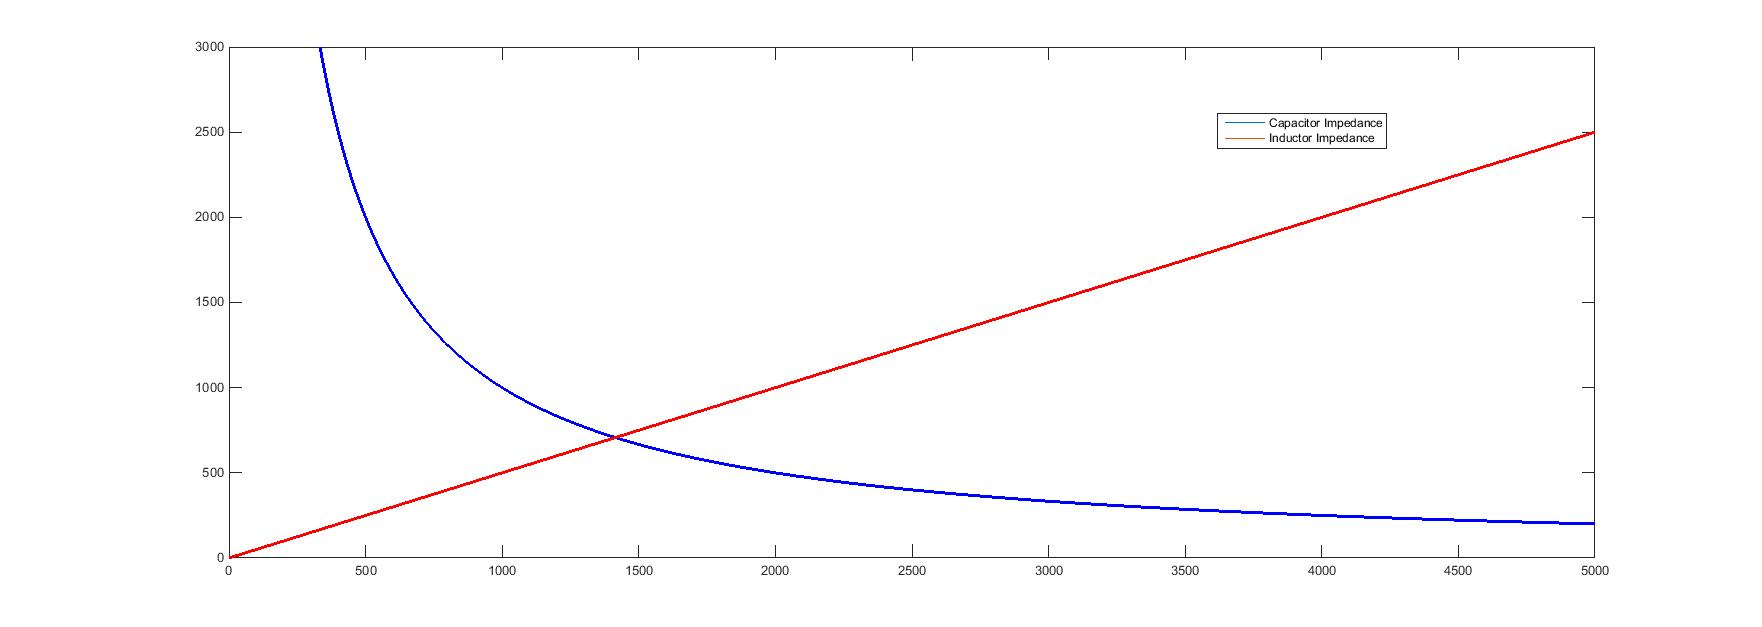
\includegraphics[width=1\textwidth]{ImpedanceVsFreq.jpg}
\end{figure}
}

This is consistanct with what we know about capacitors and inductors for DC ($\omega =0$).  A capacitor is a open circuit ($Z=\infty$) and an inductor is a short ($Z=0$).
\newpage
\clearpage
\pagebreak
\textbf{Example 5}--- For the circuit shown in Figure \ref{fig: Example5}, find the impedance of the box if $v(t) = 50\cos(500t)\  V$ and $i(t)= 4\cos(500t-60^o)\ A$.

\begin{figure} [h!]
\centering
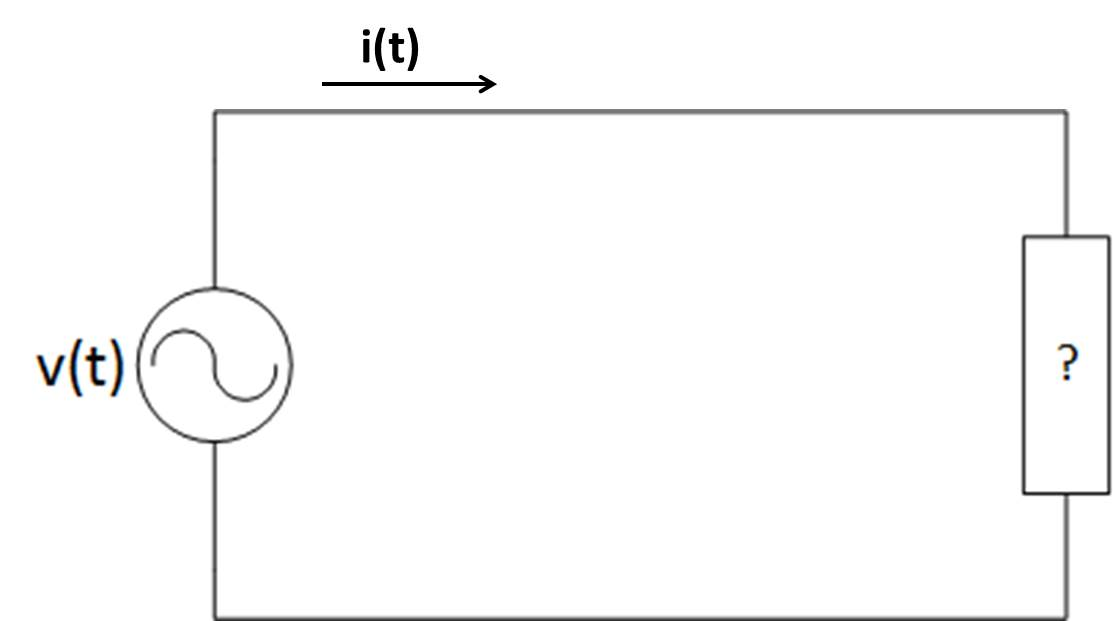
\includegraphics[width=0.5\textwidth]{Example5.jpg}
\caption{Circuit to accompany Example 5}
\label{fig: Example5}
\end{figure}

\soln{6in}{
Step 1 - Write voltage and current as phasors
\[
\mathbf{V} = 50\angle 0^o = 50
\]
\[
\mathbf{I} = 4\angle(-60^o) = 2-j3.46
\]
Step 2 - Use $\mathbf{V} = \mathbf{I}Z$ to find the impedance
\[
Z = \frac{\mathbf{V}}{\mathbf{I}}= \frac{50}{4\angle(60^o)} = 12.5\angle 60^o = 6.25 +j10.8\ \Omega
\]
}



\newpage
\clearpage
\pagebreak

\newpage
\clearpage
\pagebreak

\newpage
\clearpage
\pagebreak






\end{document}


% Equation Array Example Code
%\begin
%{eqnarray}
%P_R &=& i_R^2R \nonumber \\
%P_R &=& (100\ mA)^2 \times 100\ \Omega \nonumber \\
%P_R &=& (100 \times 10^{-3}\ A)^2 \times 100\ \Omega \\
%P_R &=& 10000 \times 10^{-6}\ A^2  \times 100\ \Omega \nonumber \\
%P_R &=& 1\ W  \nonumber
%\end{eqnarray}

% Figure Example Code
%\begin{figure} [h!]
%\centering
%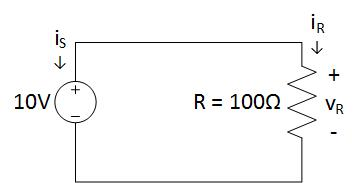
\includegraphics[width=0.5\textwidth]{OhmsLawExampleSolution.jpg}
%\caption{Ohm's Law example circuit}
%\label{fig: OhmsLawExampleSolution}
%\end{figure}

%Table Example Code
%\begin{table}[h]
%\centering
%\begin{tabular}{|l|c|c|}
%\hline
%Prefix & Abbreviation & Value \\
%\hline \hline
%Giga & $G$ & $10^9$ \\
%Mega & $M$ & $10^6$ \\
%Kilo & $k$ & $10^3$ \\
%\hline
%milli & $m$ & $10^{-3}$ \\
%micro & $\mu$ & $10^{-6}$ \\
%nano & $n$ & $10^{-9}$ \\
%pico & $p$ & $10^{-12}$ \\
%\hline
%\end{tabular}
%\caption{Engineering prefixes and values}
%\label{tab: Eng Prefixes}
%\end{table}
